\chapter{Las tipologías de TFG y su desarrollo}
\label{cap:Tipologías}

% -> Alberto: 
% Sugiero sacarlo del texto y meterlo como Anexo (o incluso ni eso) lo hablamos en reunión

% María José: lo he puesto directamente en el capítulo 4. Sugiero quitar este capítulo.

% Comentarios: Meter una introducción a las diferentes topologías, antes de entrar en profundidad a cada una de ellas, indicando también que existen otras tipologías menos comunes incluso híbridas.
% Descripción detallada de cada uno de los elementos que tienen que aparecer en la documentación.
% Ejemplo para un desarrollo clásico de software. Variaciones y desarrollo ágil (por ejemplo, siguiendo Scrum).

%Están comentadas las section porque ya vienen incluidas en los inputs
%\section{TFG de desarrollo de software} %Maria Jose
\section{TFG de Desarrollo de Software}
\label{apendice:desarrollo}
% María José

Existe una modalidad de TFG que es la de desarrollo de software, cuyo objetido será la creación de una aplicación o biblioteca en el contexto de un problema determinado. El objetivo de esta sección será explicar brevemente cómo llevar a cabo la elaboración de la memoria si tu TFG es de este tipo.

Lo primero que debes hacer es decidir qué metodología de desarrollo o ciclo de vida seguirás. Tienes varias opciones que pasamos a describir brevemente, pues seguro las has visto con más detalle en una o varias asignaturas de la carrera: 
\begin{itemize}
    \item \textbf{Ciclo de vida clásico o en cascada}: los requisitos se establecen al inicio y no cambian, se realizan secuencialmente las fases de diseño, implementación y pruebas, y los resultados se ven cuando el proyecto está ya avanzado. 
     \item \textbf{Metodología ágil}: se establecen iteraciones en las que se van se van agregando nuevas funcionalidades a la aplicación final. En cada iteración se realizan tareas de especificación, diseño, implementación y pruebas. El usuario final puede ir viendo y probando los resultados al final de cada iteración e intervenir para mejorar. Ejemplo: SCRUM.
     \item \textbf{Espiral o de Riesgos}: consiste en cuatro etapas: planificación, análisis de riesgo, desarrollo de prototipo y evaluación del cliente. Se puede volver de cada etapa a las anteriores en caso de que haya que modificar algo y antes de seguir con las siguientes etapas. Conviene para proyectos en los que se han previsto inicialmente riesgos económicos o técnicos, como la seguridad, que hay que gestionar si se quiere que el proyecto llegue a buen término.
     \item \textbf{Dirigida por pruebas}: primero se diseñan las pruebas, pensando en los requisitos que puede ser más difícil de abordar, principalmente los no funcionales, luego se completan los requisitos y se escribe un código. A continuación se realizan las pruebas planificadas y después se refactoriza el código para mejorarlo. Todo este proceso se hace de forma iterativa, abordando en cada iteración diferentes pruebas y requisitos. Ejemplo: Test Driven Development (TDD).

\end{itemize}

Existen otras metodología más específicas, según el tipo de desarrollo que vas a realizar, como la DevOps, en la que los  equipos de desarrollo  de software y los equipos de operaciones de la empresa (como el de marketing, contabilidad o gestión de almacén, por ejemplo) trabajen juntos, facilitando la comunicación e integrando mejor las tareas de ambos. También hay metodologías específicas para el diseño de videojuegos, que incluyen fases para el diseño de \textit{storyboards}, y diferencian la creación de personajes, escenas, narrativa, etc. Igual ocurre con metodologías que impliquen el diseño o uso de hardware (como tarjetas, placas, dispositivos del tipo Blackberry Pi, o sensores), se suelen incluir algunas fases de diseño, construcción y prueba del hardware. 


Sea cual sea la metodología que escojas, debes justificar su elección en la memoria, bien en el capítulo del estado del arte,  revisando y comparando varias, o bien en el capítulo de tu propuesta, antes de empezar a dar detalles del desarrollo. En la carrera has visto varias asignaturas relacionadas con ingeniería del software y has aprendido varias metodologías y herramientas. Es el momento de aplicarlas en un proyecto completo. Te aconsejamos que las valores, y desde el principio escojas una, y llegues a un acuerdo sobre ella con la persona que te tutoriza. La planificación temporal del proyecto debe tener en cuenta esta metodología en la parte del desarrollo para asignar tiempos a todas sus fases o iteraciones. 

En el capítulo de tu propuesta te aconsejamos que incluyas una sección para cada una de las fases del ciclo de vida que sigas. En el caso de metodologías ágiles, incluye una primera sección con el \textit{Product Backlog} (la lista de historias de usuario priorizadas y organizadas en iteraciones) y luego una sección por cada iteración, explicando en cada una las tareas de especificación, diseño, implementación y pruebas que llevas a cabo.

Es muy importante que en la memoria utilices herramientas de ingeniería del software como las que te han enseñado en la carrera, que ayudan a visualizar diversos aspectos del desarrollo, del tipo diagramas de casos de uso, plantillas de casos de uso o de historias de usuario, diagramas de arquitectura del sistema, de clases, de secuencia, de actividad, de la estructura de la base de datos, etc. También puedes presentar esquemas o listas de cómo has estructurado el software: paquetes, tipos de ficheros, localización en la arquitectura del software final, etc. Si tu software tiene una interfaz que has diseñado, incluye los bocetos que has hecho, como fotografías de los dibujos en papel, o capturas de pantalla de herramientas de diseño de interfaces). 

Evita incluir código en la memoria cuando abordes la implementación, a no ser que un objetivo de tu proyecto sea la propuesta de un algoritmo específico o la realización de cambios en algoritmos existentes para su mejora. En algunos casos, puede ser interesante incluir pseudocódigo. En cualquier caso tu código debería estar en un repositorio \textit{online} (como Github o Gitlab) enlazado desde el proyecto.

Debes destacar qué tipo de pruebas realizas sobre el software: unidad, integración, rendimiento, usabilidad, etc. Da detalles sobre las pruebas que planificas, y sobre qué métodos y herramientas utilizas para realizarlas, y también sobre sus resultados. Explica las mejoras realizadas si los resultados no son los esperados. 

En algunos proyectos también se hacen pruebas finales para validar el desarrollo realizado con expertos o usuarios finales. En ese caso, incluye una sección dando detalles de estas pruebas: objetivos, participantes, procedimiento, instrumentos de evaluación, resultados y valoración final.

El profesor JJ Merelo ha escrito una serie de artículos muy interesantes sobre cómo aplicar buenas prácticas de desarrollo ágil en tu TFG \cite{TFGs2024JJ}. Échales un vistazo porque pueden serte de mucha utilidad. 

Para finalizar, si durante el desarrollo has encontrado problemas que has tenido que solucionar, dale visibilidad a ese trabajo describiendo las alternativas de solución que has explorado y explicando la solución escogida para que otra persona que lea tu memoria pueda beneficiarse de ella. Si ha quedado algún problema por resolver, indica el motivo. Puede ser interesante que al final del capítulo de propuesta incluyas una sección sobre esto para mostrar tus capacidades de resolución de problemas y toma de decisiones como ingeniero o ingeniera. 

Y ten en cuenta que tu TFG puede ser una gran excusa para aprender cosas nuevas. Si en el grado has estudiado una metodología muy bien y la has practicado pero no has visto otra que consideres interesante y quizá útil profesionalmente y te interesaría aprender, no te quedes en tu zona de confort y aprovecha la oportunidad para aprenderla y ponerla en práctica. Tu TFG y todo lo que hayas aprendido durante el proceso de desarrollo del mismo será una magnífica carta de presentación para tu próxima etapa profesional.

%\section{TFG de Experimentación Científica} % Eugenio y Rocio
\section{TFG de investigación}
\label{appendix:investigacion}

% (Por si puede ser de interés: https://bpb-us-w2.wpmucdn.com/portfolio.newschool.edu/dist/2/14941/files/2017/06/Judith_Bell_Doing_Your_Research_Project-xhunbu.pdf)
% Se podría dar un layout genérico para seguir en un TFG de este tipo.

% \subsection{Introducción}
%OJOJOJOJOJO ¿¿¿¿¿METER ALGUNA REFERENCIA BIBLIOGRÁFICA??????
La Ingeniería Informática se centra en la aplicación de conocimientos teóricos-prácticos para ofrecer la mejor solución posible a un problema, teniendo en cuenta las dimensiones temporales, personales, materiales y económicas. La Ingeniería Informática actual cuenta con desafíos científicos de gran envergadura en cada una de sus especialidades, destacándose a continuación algunos de ellos:
\begin{itemize}
    \item los retos electrónicos de aumentar el nivel de integración de las placas de unidades de procesamiento, ya sean de datos (CPU) o especializadas en gráficos (GPU), fundamentales para continuar ampliando la capacidad de cómputo de los sistemas informáticos;
    \item el amplio y complejo reto computacional y social que representa la inteligencia artificial;
    \item el continuo empeño en mejorar todo lo relativo al procesamiento geométrico para impulsar el avance de la representación gráfica;
    \item el objetivo de conseguir una informática sostenible a través de la mejora de la aplicación de los conceptos de la informática teórica para el diseño y desarrollo de algoritmos eficientes en tiempo y en espacio;
    \item la responsabilidad de mejorar las metodologías y métodos de desarrollo para la programación de sistemas informáticos seguros, robustos y respetuosos con la privacidad de los datos.
\end{itemize}
%Sin embargo, la aplicación trasversal de la informática hace que la Ingeniería Informática esté presente en el trabajo científico diario de un amplio espectro de disciplinas, sobresaliendo la investigación en medicina, química o biología. Los retos científicos propios y ajenos a los que se tiene que enfrentar la Ingeniería Informática, obliga al graduado a disponer de unas mínimas habilidades científicas, que le permitan aplicar los principios de la Ingeniería Informática al método científico, y contribuir, de esta forma, al progreso científico de cualquier disciplina.

La Ingeniería Informática es una disciplina muy transversal, por tanto, tenemos el reto de ser excelentes dentro de nuestro propio campo y, además, debemos aprender y conocer el dominio del problema donde aplicaremos la solución. En el contexto de un trabajo de investigación, adicionalmente, tendremos que respetar las pautas del método científico. 

%La Ingeniería Informática, al igual que otras ingenierías, trasciende las fronteras clásicas de la ingeniería. E, es decir, a la aplicación de conocimientos teórico-prácticos para ofrecer la mejor solución posible a un problema con unas restricciones temporales, personales, materiales y económicas. La Ingeniería Informática actual cuenta con desafíos científicos de gran envergadura en cada una de sus especialidades, destacándose a continuación algunos de ellos: los retos electrónicos de aumentar el nivel de integración de las placas de unidades de procesamiento, ya sean de datos (CPU) o especializadas en gráficos (GPU), fundamentales para continuar ampliando la capacidad de cómputo de los sistemas informáticos; el amplio, ilusionante y complejo reto computacional y social que representa la inteligencia artificial; el continuo empeño en mejorar todo lo relativo al procesamiento geométrico para impulsar el avance de la representación gráfica; el objetivo de conseguir una informática sostenible a través de la mejora de la aplicación de los conceptos de la informática teórica para el diseño y desarrollo de algoritmos eficientes en tiempo y en espacio; la responsabilidad de mejorar las metodologías y métodos de desarrollo para la programación de sistemas informáticos seguros, robustos y respetuosos con la privacidad de los datos; o el desafío de mejorar las metodologías de trabajo con el fin de que la Informática continúe avanzando con una verdadera ingeniería. Sin embargo, la aplicación trasversal de la informática, hace que la Ingeniería Informática esté presente en el trabajo científico diario de un amplio espectro de disciplinas, sobresaliendo la investigación en medicina, química o biología. Los retos científicos propios y ajenos a los que se tiene que enfrentar la Ingeniería Informática, obliga al graduado en Ingeniería Informática a disponer de unas mínimas habilidades científicas, que le permitan aplicar los principios de la Ingeniería Informática al método científico, y contribuir de esta forma al progreso científico de cualquier disciplina.

La tipología de {\it TFG de Experimentación Científica} representa la oportunidad de aplicar los conocimientos adquiridos durante el grado a la resolución de un problema científico en el que interviene una metodología informática o sistema computacional, y por tanto demostrar y ampliar el desarrollo de las habilidades científicas del futuro graduado en Ingeniería Informática.
%La tipología de TFG de experimentación científica representa la oportunidad de aplicar los conocimientos adquiridos durante el grado a la resolución de un problema científico en el que interviene una metodología informática o un sistema computacional, y por tanto de mostrar y ampliar el desarrollo de las habilidades científicas del futuro graduado en Ingeniería Informática.

Aunque pudiera parecer que en este tipo de TFG sólo se deben aplicar recomendaciones o prácticas propias de la actividad científica, no se debe olvidar que este TFG es indispensable para la obtención de un título de graduado en ingeniería. Por tanto, además de aplicar procedimientos científicos, se deben seguir y emplear principios de ingeniería, y sobre todo los propios de la Ingeniería Informática estudiados durante la carrera.
%Aunque pudiera parecer que en este tipo de TFG solo se deben aplicar recomendaciones o prácticas propias de la actividad científica, no se debe olvidar que este TFG es indispensable para la obtención de un título de graduado en ingeniería. Por tanto, además de aplicar procedimientos científicos, se deben seguir y emplear principios de ingeniería, y sobre todo los propios de la Ingeniería Informática estudiados durante la carrera.

Las recomendaciones sobre el tipo de TFG de Experimentación Científica se expondrán de la siguiente manera: primero se presentará el \textit{método científico}, es decir, elemento diferenciador de este tipo de TFG y que debe guiar su elaboración (véase la sección \ref{tfx_inv_s_met_cientifico}); posteriormente se expondrá cómo estructurar el trabajo y la memoria del TFG buscando siempre una correspondencia con el método científico (Sección  \ref{tfx_inv_s_est_trabajo_memoria}) y por último se enunciarán una serie de recomendaciones (Sección \ref{tfx_inves_ss_recomendaiones}).
%Las recomendaciones sobre el tipo de  TFG de experimentación científica se expondrán de la siguiente manera: primero se presentará el \textit{método científico}, es decir, elemento diferenciador de este tipo de TFG y que debe guiar su elaboración (v. sección \ref{tfx_inv_s_met_cientifico}); posteriormente se expondrá cómo estructurar el trabajo y la memoria del TFG buscando siempre una correspondencia con el método científico (v. sección \ref{}) y por último se enunciarán una serie de recomendaciones (v. sección \ref{}).}

\subsection{El Método Científico}\label{tfx_inv_s_met_cientifico}

La investigación es un actividad intelectual y experimental realizada de modo sistemático con el propósito de aumentar los conocimientos sobre una determinada materia\footnote{Real Academia Española - \url{http://rae.es}}. En otras palabras, la investigación busca adquirir nuevos conocimientos y/o resolver problemas teóricos o prácticos mediante una actividad metódica y \underline {reproducible}. La consecución de los objetivos de la investigación precisa de la aplicación de una determinada estrategia de trabajo, que en este caso se conoce como \textbf{método científico}. Este está constituido por una serie de actividades, que aunque se resumen en la Figura \ref{fg_met_cientifico}, se detallan a continuación:

\begin{figure}[!t]
    \centering
    \usetikzlibrary {shapes.geometric}
    % Define block styles
    \tikzstyle{decision} = [diamond, draw, fill=black!10, text width=4.5em, text badly centered, node distance=3cm, inner sep=0pt]
    \tikzstyle{block} = [rectangle, draw, fill=blue!10, minimum width=7em, text centered, rounded corners, minimum height=4em]
    \tikzstyle{arrow}=[draw, -latex]
    %\tikzstyle{cloud} = [draw, ellipse,fill=red!20, node distance=3cm, minimum height=2em]
    
    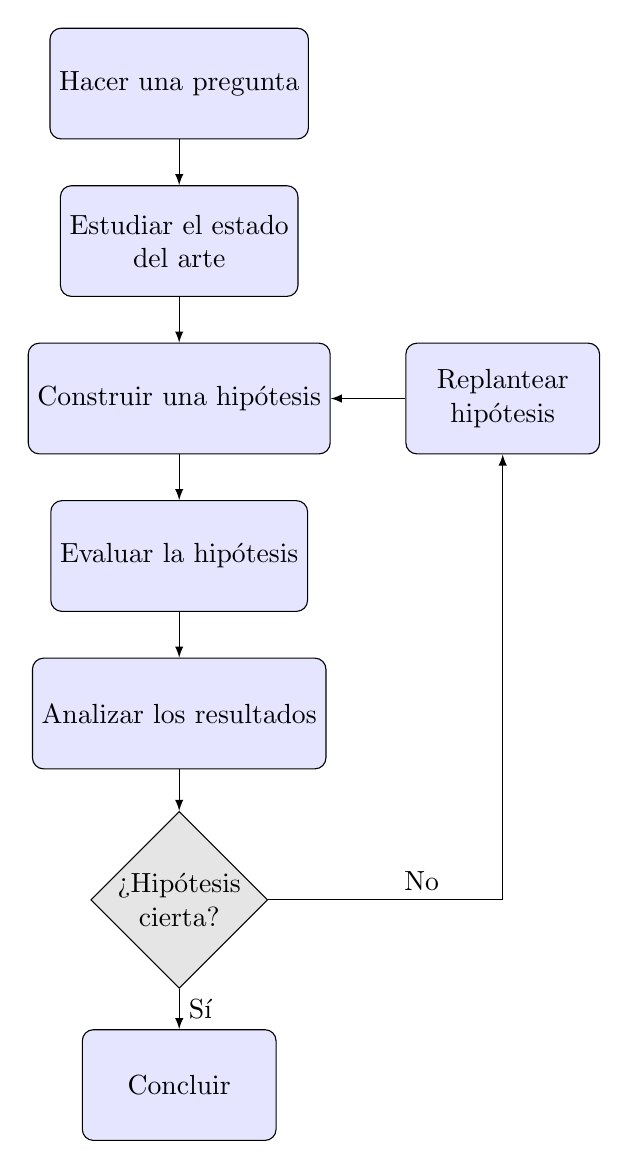
\begin{tikzpicture}[node distance = 2cm, auto]
        % Place nodes
        \node [block, align=center] (A) {Hacer una pregunta};
        \node [block, below of=A, align=center] (B) {Estudiar el estado\\del arte};
        \node [block, below of=B, align=center] (C) {Construir una hipótesis};
        \node [block, below of=C, align=center] (D) {Evaluar la hipótesis};
        \node [block, below of=D, align=center] (E) {Analizar los resultados};
        \node [block, right of=C, align=center, xshift=6em] (F) {Replantear\\hipótesis};
        \node [decision, below of=E, align=center, yshift=1.8em] (G) {¿Hipótesis cierta?};
        \node [block, below of=G, align=center, yshift=-1em] (J) {Concluir};
        % Draw edges
        \path [arrow] (A) -> (B);
        \path [arrow] (B) -> (C);
        \path [arrow] (C) -> (D);
        \path [arrow] (D) -> (E);
        \path [arrow] (F) -> (C);
        \path [arrow] (E) -> (G);
        \path [arrow] (G) -> node [text width=2.5cm, midway, right] {Sí} (J);
        \path [arrow] (G) -| node [text width=2.5cm, midway, above] {No} (F);
    \end{tikzpicture}

    %\includegraphics[width=.8\textwidth]{images/Método_científico_2021.jpg}
    \caption{Diagrama que representa el método científico.}\label{fg_met_cientifico}% \textcolor{red}{DEBE GENERARSE CON TIKZ. ESTO ES UN BORRADOR. Fuente: \url{https://es.wikipedia.org/wiki/M\%C3\%A9todo_cient\%C3\%ADfico\#/media/Archivo:M\%C3\%A9todo_cient\%C3\%ADfico_2021.jpg}}
\end{figure}

\begin{itemize}
    \item \textbf{Hacer una pregunta}. Todo trabajo científico comienza con la identificación de un problema, de una necesidad, de una carencia, en definitiva, de un ¿a qué se debe esto? o ¿cómo puedo resolver esto?, o lo que anglosajones denominan \textit{gap}. Si no existe esta pregunta, problema o necesidad, deja de tener todo sentido el invertir tiempo y esfuerzo, y por ende dinero, en la realización de una experimentación cuyo fin no está asociado a ofrecer una respuesta útil.
    %\textbf{Hacer una pregunta}. Todo trabajo científico comienza con la identificación de un problema, de una necesidad, de una carencia, en definitiva, de un ¿a qué se debe esto? o ¿cómo puedo resolver esto?, o lo que anglosajones denominan \textit{gap}. Si no existe esta pregunta, problema o necesidad, deja de tener todo sentido el invertir tiempo y esfuerzo, y por ende dinero, en la realización de una experimentación cuyo fin no está asociado a ofrecer una respuesta útil.

    \item \textbf{Estudiar el estado del arte}. La identificación de una necesidad o el surgimiento de una pregunta científica, no implica que ésta sea novedosa o que no tenga ya una respuesta. Por consiguiente, las acciones que intervienen en esta fase son: \begin{enumerate*}[label=(\arabic*)] \item identificar la disciplina científica donde se encuadra la pregunta a responder; \item analizar la novedad de la pregunta identificada, así como si ha sido ya respondida; y \item en caso de que el reto sí sea novedoso, estudiar la investigación relacionada con el ánimo de aprender los métodos ya usados, y emplearlos como inspiración en el diseño de la metodología o método original que de respuesta al desafío en estudio.\end{enumerate*}
    %\textbf{Estudiar el estado del arte}. La identificación de una necesidad o el alumbramiento de una pregunta científica, no implica que esta sea novedosa o que no tenga ya una respuesta. Por consiguiente, las acciones que intervienen en esta fase son: \begin{enumerate*}[label=(\arabic*)] \item identificar la disciplina científica donde se encuadra la pregunta a responder; \item analizar la novedad de la pregunta identificada, así como si ha sido ya respondida; y \item en caso de que el reto sí sea novedoso, estudiar la investigación relacionada con el ánimo de aprender los métodos ya usados, y emplearlos como inspiración en el diseño de la metodología o método original que de respuesta al desafío en estudio.\end{enumerate*}

    \item \textbf{Construir una hipótesis}. Una vez estudiado el estado del arte relacionado con el problema, se debe definir una hipótesis, sobre la cual se diseñará la solución y se evaluará si se confirma, y por tanto resolverá el reto, o si se desecha, y en consecuencia tener que definir otra hipótesis.
    %\textbf{Construir una hipótesis}. Una vez estudiado el estado del arte relacionado con el problema, se debe definir una hipótesis, sobre la cual se diseñará la solución y se evaluará si se confirma, y por tanto resolverá el reto, o si se desecha, y en consecuencia tener que definir otra hipótesis.

    \item \textbf{Evaluar la hipótesis}. Esta fase se compone de las siguientes acciones: \begin{enumerate*}[label=(\arabic*)]\item diseñar y desarrollar una metodología o método acorde a la hipótesis; \item diseñar un conjunto de experimentos que permitan evaluar la metodología o método desarrollado; y \item evaluar con métricas de evaluación estándares y propias del área donde se circunscribe el problema de investigación con el fin de ofrecer una evaluación objetiva y comparable. Así mismo, se recomienda ofrecer todos los detalles de desarrollo y de evaluación, con el ánimo de que la experimentación sea reproducible por cualquier investigador. Este recomendación contribuye a confiar en la experimentación realizada, en el método o metodología propuesta, a la transferencia de conocimiento y al progreso científico.\end{enumerate*}
    %\textbf{Evaluar la hipótesis}. Esta fase se compone de las siguientes acciones: \begin{enumerate*}[label=(\arabic*)]\item diseñar y desarrollar una metodología o método acorde a la hipótesis; \item diseñar un conjunto de experimentos que permitan evaluar la metodología o método desarrollado; y \item evaluar con métricas de evaluación estándares y propias del área donde se circunscribe el problema de investigación con el fin de ofrecer una evaluación objetiva y comparable. Así mismo, se recomienda ofrecer todos los detalles de desarrollo y de evaluación, con el ánimo de que la experimentación sea reproducible por cualquier investigador. Este recomendación contribuye a confiar en la experimentación realizada, en el método o metodología propuesta, a la transferencia de conocimiento y al progreso científico.\end{enumerate*}

    \item \textbf{Analizar los resultados}. Esta fase es la más determinante, porque en función de su resultado, se podrá decir que se acepta la hipótesis, y por tanto se concluye que el método o metodología desarrollados resuelven el desafío objeto de estudio, o por el contrario se rechaza la hipótesis. Este rechazo implica que se debe volver a la definición de la hipótesis, o dicho de otro modo, a modificar la hipótesis y desarrollar otro método o metodología acorde a la nueva hipótesis.
    %\textbf{Analizar los resultados}. Esta fase es la más determinante, porque en función de su resultado, se podrá decir qu se acepta la hipótesis, y por tanto se concluye que el método o metodología desarrollados resuelven el desafío objeto de estudio, o por el contrario se rechaza la hipótesis. Este rechazo implica que se debe volver a la definición de la hipótesis,  o dicho de otro modo, a modificar la hipótesis y desarrollar otro método o metodología acorde a la nueva hipótesis.
\end{itemize}

Al igual que el método científico guía la labor de los investigadores de cualquier área, también debe ser la base de un TFG de Experimentación Científica.

% ------------------------------------------------------------

%Definición de investigación.
%La investigación es un actividad intelectual y experimental realizada de modo sistemático con el propósito de aumentar los conocimientos sobre una determinada materia\footnote{Real Academia Española - \url{http://rae.es}}. En otras palabras, la investigación busca adquirir nuevos conocimientos y/o resolver problemas teóricos o prácticos mediante una actividad metódica y \underline {reproducible}. Para poder llevar a cabo una investigación exitosa es necesario tener en cuenta los siguientes elementos: 
%\begin{itemize}
%    \item Recopilar toda la información relevante sobre el problema a tratar utilizando fuentes heterogéneas y fiables.
%    \item Indagar sobre otros estudios ya realizados y publicados en la literatura científica sobre la misma problemática, analizando sus beneficios y sus limitaciones.
%    \item Seguir una metodología científica para poder así desarrollar el trabajo de manera organizada y coherente.
%    \item Mostrar los resultados obtenidos y valorarlos de forma objetiva sin omisiones.
%    \item Asegurar la reproducibilidad del trabajo, permitiendo que el tribunal o cualquier otra persona interesada sea capaz de verificarlo y replicarlo.
%\end{itemize}

%Conocimiento previo sobre el estado de la cuestión.
%Estructura del marco teórico y conceptual.
%De esta lista de elementos haremos especial hincapié en proveer de un marco teórico y conceptual que permita al tribunal, y a cualquier otro potencial lector, de la información básica necesaria para comprender la investigación realizada. De todas las tipologías de TFG de esta sección, la tipología de TFG de investigación es, probablemente, la que lleve más páginas dedicadas al estado del arte. Por tanto, también la bibliografía utilizada será más extensa. Debe de quedar claro que comprendes la temática y conoces qué cosas se han hecho ya y qué falta por hacer.

%Importancia de partir de una pregunta de partida.
%Otro punto importante a destacar en la memoria de los TFGs de investigación es la motivación del trabajo. No hay que confundir el apartado de motivación con una motivación personal. La motivación del trabajo, en este tipo de tipología de TFG, se refiere a identificar una brecha en el conocimiento actual del tema a tratar y de cómo la investigación en ese punto puede ayudar a contribuir en al área de estudio. Por tanto la motivación del trabajo debe incluirse en la memoria luego del estudio del estado del arte, ya que es muy posible que debas hacer referencia a algún punto ya tratado.

%Una vez detallado el problema de estudio y la motivación del TFG, es momento de hablar de los objetivos del trabajo. Para poder definir correctamente estos objetivos es necesario primero definir las hipótesis de partida, ya que la verificación o no de estas hipótesis serán justamente los objetivos principales del TFG. En el proceso de formulación de hipótesis debes plantear posibles respuestas a las preguntas surgidas durante tu análisis del estado del arte. Recuerda que las hipótesis deben poder ser verificables y falsables, es decir, susceptibles de ser refutadas.
   
En el siguiente apartado veremos en más detalle como llevar a cabo un TFG de Experimentación Científica siguiendo una serie de pasos que nos aseguren que los resultados obtenidos sean de fiables y de calidad.

\subsection{Estructura del Trabajo y de la Memoria}\label{tfx_inv_s_est_trabajo_memoria}

La estructura de la memoria no debe por qué distar mucho del resto de tipologías, pero sí debe recoger de forma adecuada el desarrollo científico realizado. Esto obliga a que el trabajo científico siga unas pautas coherentes que dirijan, al menos, la labor experimental de una forma ordenada y dirigida a la evaluación con éxito de la hipótesis. El método científico, presentado en la sección \ref{tfx_inv_s_met_cientifico}, es una guía muy recomendable para orientar todo la actividad experimental y la redacción de la memoria. Por ende, la memoria debe reflejar: \begin{enumerate*}[label=(\arabic*)]\item la existencia de una necesidad de investigación, \item que esta no haya sido aún resuelta, o por lo menos no completamente, \item la definición de una hipótesis, \item el análisis, diseño e implementación del método o metodología que lleve a cabo la hipótesis y \item la evaluación de esta.\end{enumerate*} A continuación, se presentará una correspondencia entre el método científico y la estructura de la memoria, que a su vez ordena todo el trabajo relacionado con esta tipología de TFG.
%La estructura de la memoria no debe por qué distar mucho del resto de tipologías, pero sí debe recoger de forma adecuada el desarrollo científico realizado. Esto obliga a que el trabajo científico siga unas pautas coherentes que dirijan, al menos, la labor experimental de una forma ordenada y dirigida a la evaluación con éxito de la hipótesis. El método científico, presentado en la sección \ref{tfx_inv_s_met_cientifico}, es una guía muy recomendable para orientar todo la actividad experimental y la redacción de la memoria. Por ende, la memoria debe reflejar: \begin{enumerate*}[label=(\arabic*)]\item la existencia de una necesidad de investigación, \item que esta no haya sido aún resuelta, o por lo menos no completamente, \item la definición de una hipótesis, \item el análisis, diseño e implementación del método o metodología que lleve a cabo la hipótesis y \item la evaluación de esta.\end{enumerate*} A continuación, se presentará una correspondencia entre el método científico y la estructura de la memoria, que a su vez ordena todo el trabajo relacionado con esta tipología de TFG.

\paragraph{Motivación - Pregunta de investigación} El primer capítulo o el capítulo de introducción del TFG debe recoger la motivación del trabajo, es decir, la razón por la cual se realiza y merece la pena esforzarse en él durante los meses que involucre su realización. Esto que, en un inicio parece complicado, consiste en encontrar un reto que tenga asociado una pregunta científica, como podría ser \textit{¿es posible la generación de texto coherente y precisa para ofrecer información sobre trastornos de la conducta alimenticia?} Si se ha llegado a esa pregunta, es que existe una necesidad ligada a una problema, que a su vez tiene un contexto. Esta conjunción de contexto, problema, necesidad y pregunta científica es lo que constituye la motivación del TFG, y la cual lo convierte en atractivo para cualquier lector, y sobre todo para la comunidad científica.
%\paragraph{Motivación - Pregunta de investigación} El primer capítulo o capítulo de introducción del TFG debe recoger la motivación del trabajo, es decir, la razón por la cual se realiza, merece la pena esforzarse en él durante los meses que involucre su realización, es interesante para cualquier lector, y representa un avance científico. Esto que parece complicado consiste en encontrar un reto que tenga asociado una pregunta científica, como podría ser \textit{¿es posible la generación de texto coherente y precisa para ofrecer información sobre trastornos de la conducta alimenticia?} Si se ha llegado a esa pregunta, es que existe una necesidad ligada a una problema, que a su vez tiene un contexto. Esta conjunción de contexto, problema, necesidad y pregunta científica es lo que constituye la motivación del TFG, y la cual lo convierte en atractivo para cualquier lector, y sobre todo para la comunidad científica.

\paragraph{Investigación relacionada - Estudiar el estado del arte} Una vez que ya se ha fijado el problema o pregunta a resolver, se deben realizar las siguientes acciones:

\begin{enumerate}
    \item \textbf{Determinar el área de investigación}. La Ingeniería Informática abarca distintas áreas científicas, por lo que lo primero es saber si la pregunta se responde desde, por ejemplo, la informática teórica, la informática gráfica, la inteligencia artificial, la electrónica, o incluso si precisa de conocimiento externo a la Ingeniería Informática, como podría ser una investigación en un dominio interdisciplinar (medicina, biología, química, etc.). Atendiendo a la pregunta anterior, si se está cuestionando sobre la posibilidad de generar automáticamente lenguaje, parece que se trataría de un problema de inteligencia artificial, dado que se pide imitar un comportamiento característico de la inteligencia humana. En este ejemplo, una vez fijada que el área es la de la inteligencia artificial, el siguiente paso sería identificar la disciplina especializada en el desafío en cuestión, que en este ejemplo sería el procesamiento del lenguaje natural, ya que es la disciplina de inteligencia artificial encargada del desarrollo de métodos y metodologías computacionales orientados a la comprensión y generación de lenguaje por parte de un ordenador.
    %\textbf{Determinar el área de investigación}. La Ingeniería Informática abarca distintas áreas científicas, por lo que lo primero es saber si la pregunta se responde desde por ejemplo la informática teórica, la informática gráfica, la inteligencia artificial, la electrónica, o incluso si precisa de conocimiento externo a la Ingeniería Informática, como podría ser una investigación en el dominio de la biología. Atendiendo a le pregunta anterior, si se está cuestionando sobre la posibilidad de generar automáticamente lenguaje, parece que se trataría de un problema de inteligencia artificial, dado que se pide imitar un comportamiento característico de la inteligencia humana como es la generación de lenguaje. Una vez fijada que el área es la de la inteligencia artificial, el siguiente paso sería identificar la disciplina especializada en el desafío en cuestión, que en este caso sería el procesamiento del lenguaje natural, ya que es la disciplina de inteligencia artificial encargada del desarrollo de métodos y metodologías computacionales orientados a la comprensión y generación de lenguaje por parte de un ordenador.

    \item \textbf{Búsqueda de los trabajos más relevantes}. Conocida el área y disciplina de investigación, es momento de encontrar los trabajos relacionados con la pregunta de investigación. En el caso particular que estamos tratando, serían modelos de generación de lenguaje. Con este dato, ya es momento de estudiar todo lo relacionado con la problemática, y seleccionar los avances más recientes. En este caso se corresponderían con los grandes modelos de lenguaje.
    %\textbf{Búsqueda de los trabajos más relevantes}. Conocida el área y disciplina de investigación, es momento de encontrar los trabajos relacionados con la pregunta de investigación. En el caso particular que estamos tratando, serían modelos de generación de lenguaje. Con este dato, ya es momento de estudiar todo lo relacionado con la problemática, y seleccionar los avances más recientes. En este caso se corresponderían con los grandes modelos de lenguaje.

    \item \textbf{Evaluación de si el reto está resuelto}. Tras la selección de los artículos más importantes es momento de evaluar si el desafío planteado está o no resuelto. En caso de que así sea, se deberá revaluar la pregunta de investigación, hasta encontrar aquella que aún no lo esté. Por contra, si no lo está, la pregunta representa un verdadero reto sobre el que merece la pena realizar el TFG.
    %\textbf{Evaluación de si el reto está resuelto}. Tras la selección de los artículos más importantes es momento de evaluar si el desafío planteado está resuelto. En caso de que así sea, se deberá revaluar la pregunta de investigación, hasta encontrar aquella que aún no lo esté. Por contra, si no lo está, la pregunta representa un verdadero reto sobre el que merece la pena trabajar.
    
    Pudiera parecer que el trabajo de esta fase termina aquí, pero no es así, porque ahora es el momento de determinar las estrategias seguidas hasta la fecha, con el fin de realizar una propuesta novedosa que pueda compararse con lo existente, y que ofrezca mejores resultados.
    %Pudiera parecer que el trabajo de esta fase termina aquí, pero no es así, porque ahora es momento de determinar las estrategias seguidas hasta la fecha con el fin de realizar una propuesta novedosa que pueda compararse con lo existente, y que ofrezca unos mejores resultados.
\end{enumerate}

El resultado de este estudio deberá reflejarse en un capítulo específico sobre el estado de la investigación asociada al proyecto. Algunos ejemplos de nombres que puede tener este capítulo son: contexto, estado de arte, estado de la cuestión, trabajos relacionados o el nombre específico de la disciplina de investigación asociada al desafío científico del TFG.
%El resultado de este estudio deberá reflejarse en un capítulo específico sobre el estado de la investigación asociada al proyecto. Algunos ejemplos de nombres que puede tener este capítulo son: contexto, estado de arte, estado de la cuestión, trabajos relacionados o el nombre específico de la disciplina de investigación asociada al desafío científico del TFG.

\paragraph{Hipótesis} Un conocimiento profundo del problema científico asociado prepara para la enunciación de la hipótesis del TFG. Esta es una suposición de estrategia, metodología o modelo a desarrollar para resolver el desafío científico en el que se está trabajando. Así mismo, si la evaluación de la hipótesis la confirma, conlleva haber propuesto una solución válida al reto científico del TFG. Automáticamente se podría pensar que un resultado negativo implica el fracaso del trabajo científico desarrollado. Esto no tiene por qué ser así, dado que de los resultados negativos también se pueden obtener conclusiones positivas, que incluso pueden servir de base para posteriores avances científicos.
%\paragraph{Hipótesis} Un conocimiento profundo del problema científico asociado prepara para la enunciación de la hipótesis del TFG. Esta es una suposición de estrategia, metodología o modelo a desarrollar para resolver el desafío científico en el que se está trabajando. Así mismo, si la evaluación de la hipótesis la confirma, conlleva haber propuesto una solución válida al reto científico del TFG. Automáticamente se podría pensar que un resultado negativo implica el fracaso del trabajo científico desarrollado. Esto no tiene por qué ser así, dado que de los resultados negativos también se pueden obtener conclusiones muy positivas, que incluso pueden servir de base para posteriores avances científicos.

La hipótesis se recomienda que también se indique en el capítulo de introducción, ya que va asociada a la pregunta de investigación. Así mismo, una vez formulada la hipótesis, ya se puede establecer los objetivos e hitos del TFG, los cuales son una forma de concretar el trabajo a realizar.
%La hipótesis se recomienda que también se indique en el capítulo de introducción, porque va asociada a la pregunta de investigación. Así mismo, una vez formulada la hipótesis, ya se puede establecer los objetivos e hitos del TFG, los cuales son una forma de concretizar el trabajo a realizar.

\paragraph{Desarrollo - Evaluación de la hipótesis} Para poder probar la validez de la hipótesis, antes hay que desarrollar la metodología o método subyacente a la misma. Por tanto, se debe comenzar primeramente con el diseño del marco experimental. En la mayoría de los casos el marco experimental va a seguir los cánones de la investigación cuantitativa, la cual requiere de una evaluación empírica. Esto obliga a seleccionar el conjunto o conjuntos de datos sobre los que realizar la evaluación, y a determinar las medidas de evaluación a utilizar
%\paragraph{Desarrollo - Evaluación de la hipótesis} Para poder probar la validez de la hipótesis, antes hay que desarrollar la metodología o método subyacente a la misma. Por tanto, se debe comenzar primeramente con el diseño del marco experimental. En la mayoría de los casos, el marco experimental va a seguir los cánones de la investigación cuantitativa, la cual requiere de una evaluación empírica. Esto obliga a seleccionar el conjunto o conjuntos de datos sobre los que realizar la evaluación, y a determinar las medidas de evaluación a usar.

La elección del conjunto de datos es una decisión muy importante del proceso de evaluación, porque si estos no son de calidad, o no son representativos, la calidad y credibilidad del marco experimental se verá resentido. En cualquier caso, siempre hay que describir los datos elegidos, y en caso de que no sean propios hacer referencia a su fuente. A continuación te mostramos algunos ejemplos de conjuntos de datos que se pueden usar:
%La elección del conjunto de datos es una decisión muy importante del proceso de evaluación, porque si estos no son de calidad o no son representativos, la calidad y credibilidad del marco experimental se verá resentido. En cualquier caso, siempre hay que describir los datos elegidos, y en caso de que no sean propios hacer referencia a su fuente. A continuación algunos ejemplos de conjuntos de datos que se pueden usar:

\begin{itemize}
    \item {\bf Conjuntos de datos externos}: Si trabajas con conjuntos de datos públicos y ampliamente conocidos por la comunidad científica es sencillo hacer referencia a ellos en la memoria. Se recomienda utilizar una tabla para mostrar comparativamente los distintos conjuntos de datos empleados, como en el ejemplo de la Tabla \ref{tab:uci}. Puedes incorporar a la tabla las columnas que sean necesarios y que incluyan toda la información sobre la cual haces referencia en el texto principal de la memoria. Presta atención a el texto que acompaña a la tabla en donde se indica tanto el origen de los datos como una cita o referencia on-line a ellos. 

\begin{table}[!ht]
\centering
\begin{tabular}{cccccc}
\hline
 & \textbf{No. de} & \textbf{No. de} & \multicolumn{3}{c}{\textbf{No. de Atributos}} \\
{\it \textbf{Dataset}} & \textbf{Casos} & \textbf{Clases} & \textbf{Nominal} & \textbf{Numérico} & \textbf{Perdidos}\\ \hline
Anneal & 898 & 6 & 32 & 6 & 29 \\
Breast Cancer & 286 & 2 & 9 & 0 & 2 \\
Diabetes & 768 & 2 & 8 & 0 & 8 \\
Heart-C & 303 & 5 & 7 & 6 & 2 \\
Hepatitis & 155 & 2 & 13 & 6 & 15 \\
House Votes & 435 & 2 & 16 & 0 & 16 \\
Iris & 150 & 3 & 0 & 4 & 0 \\
Lymphography & 148 & 4 & 15 & 3 & 0 \\
Vowel & 990 & 11 & 3 & 10 & 0 \\
Wine & 178 & 3 & 0 & 13 & 0 \\
Zoo & 101 & 7 & 16 & 1 & 0 \\
\hline
\end{tabular}
\caption{Conjuntos de datos utilizados en este trabajo provenientes del repositorio UCI (\url{https://archive.ics.uci.edu/}).\label{tab:uci}}
\end{table}

    \item {\bf Conjuntos de datos propios}: si dentro de tu propuesta de trabajo incluyes la generación de conjuntos de datos artificiales propios, entonces necesitas crear un apartado en la memoria para detallar todo el proceso. Si por otro lado, el conjunto de datos te lo ha dado tu tutor, entonces necesitas detallar su origen y características. Si es posible incluye el o los conjuntos de datos al entregar la memoria. Si por alguna razón los datos son privados o no tienes permiso para difundirlos debes entonces explicarlo detalladamente. Recuerda que para trabajar con datos con información de carácter personal, antes debes anonimizarlos. 
    \item {\bf Conjuntos de datos artificiales}: si cuentas con conjuntos de datos creados artificialmente, también llamados datos sintéticos, debes explicar cómo se han generado. Si el procedimiento de generación de estos datos es propuesta tuya, entonces descríbelo con detalle como se explica en el apartado anterior. En caso de ser generados por terceras partes entonces alcanza con referenciar ese trabajo y explicar brevemente cómo se realiza este proceso. Igualmente para ambos casos necesitas mostrar en una tabla una descripción de los conjuntos de datos, como puedes ver en la Tabla \ref{tab:fake}. Recuerda que tu trabajo debe de poder ser reproducible por cualquier persona, por tanto debes incluir en el material a entregar los conjuntos de datos que hayas generado tú o un enlace a aquellos generados por terceras personas.

\begin{table}[!ht]
\centering
\label{tab:results}
\begin{tabular}{c|ccc}
\hline
{\it \textbf{Dataset}} & \textbf{Edificio} & \textbf{Árbol} & \textbf{Persona} \\
\hline
Sintético A & 5 & 10 & 4 \\
Sintético B & 0 & 12 & 11 \\
Sintético C & 1 & 2 & 2 \\
Sintético D & 3 & 2 & 3 \\
Sintético E & 4 & 5 & 1 \\
\hline
\end{tabular}
\caption{Elementos incluidos en los distintos conjuntos de datos generados artificialmente.\label{tab:fake}}
\end{table}
\end{itemize}

El siguiente paso es \textbf{diseñar e implementar la metodología o modelo}. Se podría decir que esta parte del TFG es para la que está más preparado el estudiante, por ser la de mayor contenido técnico. El diseño y desarrollo deben seguir los principios de ingeniería aprendidos durante la carrera, siendo recomendable que el alumno tome decisiones en el ámbito de elección de lenguaje de programación, de bibliotecas a usar y de entorno de programación a utilizar.
%El siguiente paso es \textbf{diseñar e implementar la metodología o modelo}. Se podría decir que esta parte del TFG es para la que está más preparado el alumno, por ser la de mayor contenido técnico. El diseño y desarrollo deben seguir los principios de ingeniería aprendidos durante la carrera, siendo recomendable que el alumno tome decisiones en el ámbito de elección de lenguaje de programación, de librerías a usar y de entorno de programación a utilizar.

Antes de proseguir, nos gustaría hacerte la recomendación de que este tipo de TFG estuvieran acompañados de un demostrador, es decir, de integrar la propuesta científica en un sistema informático que muestre su utilidad. Si se opta por ello, el desarrollo del demostrador debe seguir las recomendaciones de la ingeniería del software, lo que implica: \begin{enumerate*}[label=(\arabic*)]\item elección de metodología de trabajo, \item realización de fase de análisis, \item diseñar la solución, \item implementar el diseño y \item validar y evaluar el software desarrollado.\end{enumerate*} Es muy recomendable la realización de un demostrador, porque permite que el alumno muestre los conocimientos adquiridos durante la carrera, sobre todo los relativos a los procesos y principios de la ingeniería del software.
%Ante de proseguir, quisiera hacerse la recomendación de que este tipo de TFG estuvieran acompañados de un demostrador, es decir, de integrar la propuesta científica en un sistema informático que muestre su utilidad. Si se opta por ello, el desarrollo del demostrador debe seguir las recomendaciones de la ingeniería del software, lo que implica: \begin{enumerate*}[label=(\arabic*)]\item elección de metodología de trabajo, \item realización de fase de análisis, \item diseñar la solución, \item implementar el diseño y \item validar y evaluar el software desarrollado.\end{enumerate*} Es muy recomendable la realización de un demostrador, porque permite que el alumno muestre los conocimientos adquiridos durante la carrera, sobre todo los relativos a los procesos y principios de la ingeniería del software.

Una vez concluida la implementación de la metodología o modelo pasamos a la fase de evaluación. Ésta debe realizarse con las medidas de evaluación usadas en los trabajos de investigación relacionados. Esto es relevante porque permite comparar la propuesta del TFG con la literatura, y así poder saber si la propuesta representa realmente un avance o no. Además, se recomienda facilitar la comparación con el estado del arte por medio de una tabla comparativa con los modelos más relevantes. No olvidar que para poder decir, por ejemplo, que un algoritmo es mejor que otro, es necesario no solo realizar múltiples experimentos, sino también someter los resultados obtenidos a análisis estadísticos. Recuerda que los experimentos que realizas deben de poder reproducirse, por tanto no olvides fijar una semilla para que, en caso de usar un generador de números aleatorios, tu trabajo sea reproducible.
%Una vez concluida la implementación de la metodología o modelo se debe evaluar. La evaluación debe realizarse con las medidas de evaluación usadas en los trabajos de investigación relacionados. Esto es relevante porque permite comparar la propuesta del TFG con la literatura, y así poder saber si la propuesta representa realmente un avance o no. Además, se recomienda facilitar la comparación con el estado del arte por medio de una tabla comparativa con los modelos más relevantes.

En cuanto a la organización de la evaluación de la hipótesis en varias secciones o capítulos, dependerá de su extensión y de si se realiza un sistema demostrador. En el caso de que se haga un sistema informático, se recomienda separar en capítulos las distintas fases del proceso de desarrollo de software. En caso contrario, puede que solo sea necesario elaborar un capítulo describiendo todo lo relativo a la elección de datos, implementación y evaluación.
%En cuanto a la organización de la evaluación de la hipótesis en capítulos, todo va a depender de su extensión y de si se realiza un sistema demostrador. En el caso de que se haga un sistema informático, se recomienda separar en capítulos las distintas fases del proceso de desarrollo de software. En caso contrario, puede que solo sea necesario elaborar un capítulo describiendo todo lo relativo a la elección de datos, implementación y evaluación.

\paragraph{Análisis de los resultados.} El análisis de los resultados y la comparación con el estado del arte es el momento decisivo de esta tipología de TFG, debido que determina si la hipótesis se acepta o no. En el caso de que se acepte, el trabajo no concluye aquí, ya que se recomienda realizar un análisis tanto de los aciertos, como de los errores que se hayan producido, dado que estos permitirán realmente entender cómo el modelo o metodología desarrollados están dando respuesta al reto de investigación.
%\paragraph{Análisis de los resultados} El análisis de los resultados y la comparación con el estado del arte es el momento decisivo de esta tipología de TFG, debido que determina si la hipótesis se acepta o no. En el caso de que se acepte, el trabajo no concluye aquí, ya que se recomienda realizar un análisis tanto de los aciertos, como de los errores que se hayan producido, dado que estos permitirán realmente entender cómo el modelo o metodología desarrollados están dando respuesta al reto de investigación.

En caso de que la hipótesis sea rechazada, se debe evaluar si un análisis profundo de los resultados puede ser interesante para la comunidad investigadora, y por tanto constituir una contribución importante para el TFG. Este análisis puede concluir que se deben elegir otros datos, que el reto ha llegado a un escenario de resultados tope, que la estrategia algorítmica no es la adecuada y que se deben seguir otras, o que la elección de las características y los parámetros de configuración del algoritmo no han sido los óptimos. Esto que pudiera parecer una fracaso, puede ser la base de futuros progresos porque ofrece a la comunidad científica un conjunto de lecciones aprendidas a tener en cuenta para posteriores desarrollos. Ahora bien, se remarca que cuando se ha obtenido un resultado negativo, el análisis de resultados debe ser profundo y con conclusiones interesantes para considerarlo como una contribución y como un TFG válido.
%En caso de que la hipótesis sea rechazada, se debe evaluar si un análisis profundo de los resultados puede ser interesante para la comunidad investigadora, y por tanto constituir una contribución importante para el TFG. Este análisis puede concluir que se deben elegir otros datos, que el reto ha llegado a un escenario de resultados tope, que la estrategia algorítmica no es la adecuada y que se deben seguir otras o que la elección de las características y los parámetros de configuración del algoritmo no han sido los óptimos. Esto que pudiera parecer una fracaso, puede ser la base de futuros progresos porque ofrece a la comunidad científica un conjunto de lecciones a tener en cuenta para posteriores desarrollos. Ahora bien, se remarca que cuando se ha obtenido un resultado negativo, el análisis de resultados debe ser profuso y con conclusiones interesantes para considerarlo como una contribución y como TFG válido.

También es posible que los experimentos realizados tengan ciertas limitaciones que afecten a la interpretación de los resultados obtenidos. Debes, por tanto, abordar este tema de manera transparente. Las limitaciones son características del diseño o metodología que influyen en la validez, aplicabilidad o generalización de los hallazgos. Pueden derivarse del diseño inicial del estudio, del método utilizado o de desafíos imprevistos durante el proyecto. Existen distintos tipos de limitaciones, como las relacionadas con el diseño o la metodología del estudio, o bien de los datos en sí, que pueden presentar problemas de calidad, disponibilidad o fiabilidad. Reconocer estas limitaciones te da la oportunidad para proponer formas de abordar estas limitaciones y demuestra un pensamiento crítico.

\paragraph{Conclusiones} El último capítulo debe ser el de conclusiones, que no debe ser una mera recapitulación del TFG, sino un lugar donde destacar si la propuesta permite aceptar la hipótesis, y los principales resultados del análisis a modo de lecciones aprendidas. En resumen, unas conclusiones que aporten valor al TFG. Adicionalmente puede ser útil contar con una lista de trabajos futuros en donde el estudiante pueda demostrar que ha comprendido el problema sobre el que ha trabajado y proponga líneas de trabajo futuras a partir de sus conclusiones.
%\paragraph{Conclusiones} El último capítulo debe ser el de conclusiones, que no debe ser una mera recapitulación del TFG, sino un lugar donde destacar si la propuesta permite aceptar la hipótesis, y los principales resultados del análisis a modo de lecciones aprendidas. En resumen, unas conclusiones que aporten valor al TFG.


%Muchos de los algoritmos que se utilizan para minería de datos tienen una componente aleatoria. Esto quiere decir que dependiendo de la semilla del generador de números aleatorios utilizado puede darnos una respuesta diferente. Para evitar tener este sesgo es necesario ejecutar varias veces el mismo algoritmo utilizando distintas semillas. Normalmente se suele ejecutar unas 5 o 10 veces y luego tomar para cada métrica a medir su media y desviación estándar. De esta manera puedes deducir si el algoritmo es robusto, si tiene mucha variabilidad, etc. Por tanto, a la hora de reportar los resultados debes incluir tanto la media como la desviación estándar en la tabla de resultados, como puedes ver en la Tabla \ref{tab:sd}.

%\begin{table}[htbp]
%\centering
%\label{tab:cityscapes}
%\begin{tabular}{c|c|c|c}
%\hline
%\textbf{Método} & \textbf{Iris} & \textbf{Diabetes} & \textbf{Ionosphere} \\ 
%\hline
%K-means & 214 (289) & 2628 (175) & 805 (202) \\
%LKM & 169 (10) & 1691 (47) & 908 (34) \\ 
%DE-LKM &  1938 (151) & 7425 (214) & 9449 (55) \\
%LC-LKM & 3764 (2431) & 12797 (44) & 17653 (2298) \\
%EM & 255 (139) & 3033 (226) & 1688 (1301) \\
%\hline
%\end{tabular}
%\caption{Tiempo de ejecución en ms. (media y desviación estándar entre paréntesis) de las 10 ejecuciones de cada %algoritmo por conjunto de datos.\label{tab:sd}}
%\end{table}

%También es necesario realizar un proceso de entrenamiento o {\it training} y uno de prueba o {\it test} posterior. Para ello se puede dividir el conjunto de datos en una parte para training y otra para test. Sin embargo, la opción más recomendada es utilizar algún tipo de validación cruzada que divide el conjunto de datos original en varias partes. Luego se utilizan todas menos una para entrenar y la restante para validar. Esto se realiza tantas veces como divisiones del conjunto de datos original hemos hecho. Finalmente se reporta la media y la desviación estándar de las métricas evaluadas. En caso de utilizar particiones ya realizadas por terceros indícalo e incluye una referencia en la memoria y/o los ficheros mismos al entregarla.

\subsection{Recomendaciones}\label{tfx_inves_ss_recomendaiones}
%Sugerencias para futuros investigadores.
%Áreas de mejora o posibles extensiones del estudio.

A modo de buenas prácticas para la realización de este tipo de TFG, se proponen a continuación una seria de consejos que esperamos que sean de utilidad:
%A modo de buenas prácticas para la realización de este tipo de TFG, se proponen una seria de consejos que se estiman que allanarán su elaboración.

\begin{itemize}
    \item \textbf{Sistema demostrador}. Como ya se ha indicado, se recomienda realizar un sistema informático que integre la propuesta científica, con el fin de que el alumno aplique los principios de ingeniería de software adquiridos durante la carrera. 
    
    \item \textbf{Manual de instalación y uso}. En caso de no realizar un sistema demostrador, es esencial proveer de toda la información necesaria para asegurar la reproducibilidad de los resultados. Eso incluye un manual de instalación y uso, el código fuente utilizado, etc.

    \item \textbf{Experimentación y redacción en paralelo}. Es práctica común de los estudiantes el realizar primero la experimentación y posteriormente la redacción de la memoria. Esto suele conllevar agobio y hastío, dado que suele apetecer más el programar un sistema informático que redactar una memoria. Por tanto, para facilitar el proceso de redacción, y también para que este sea más rico, se recomienda realizar la tarea de experimentación y redacción en paralelo.

    \item \textbf{Registrar todo paso de la experimentación}. Es importante registrar todo paso del proceso científico que se realice, dado que facilitará luego su desarrollo en la memoria. Esto incluye el uso de sistemas de control de versiones, llevar un \textit{log} donde se detallen los distintos experimentos realizados, etc.

    \item \textbf{Continua interacción con la persona que te tutoriza}. Teniendo en cuenta que la metodología de investigación te puede resultar novedosa, es muy importante que tengas reuniones con tu tutor o tutora frecuentes con objeto de que te vaya guiando paso a paso por ella y en las que tendrás que aprovechar para consultar todas las dudas que te vayan saliendo.

    \item \textbf{Trabajos futuros}. La investigación es un proceso continuo donde cada investigador aporta su pequeño grano de arena. A medida que uno se sumerge dentro del área de estudio, van surgiendo nuevas ideas e hipótesis que por la extensión y cantidad de horas para realizar el TFG no pueden ser acometidas. Es importante por tanto dejarlas por escrito, en el apartado de conclusiones o uno propio, de forma que cualquier lector pueda retomar el trabajo realizado y extenderlo desde el punto en donde ha acabado el TFG.

    \item \textbf{Reproducibilidad}. Aunque ya se ha comentado en esta sección el tema de la reproducibilidad, es importante hacer hincapié en ella. Es muy importante que describas tu investigación con tal detalle que cualquier otra persona pueda reproducir de manera fehaciente todo el proceso que has realizado y obtener los mismos resultados. De esta forma podrá comparar sus propios resultados con los tuyos. Por desgracia, aunque es verdad que cada vez menos, te encontrarás con situaciones en las que te interesaría evaluar un modelo que ya ha sido publicado pero no tienes suficientes detalles para implementarlo tú o no aportan información de valores de parámetros con los que han obtenido los resultados que se han publicado. Estas situaciones son bastante frustrantes pues, aunque el modelo sea interesante, similar al tuyo, utilice el mismo enfoque, o cualquier otra causa, no podrás emplearlo para comparar resultados. Por tanto, describe tus modelos y entornos experimentales con todo detalles. Incluso pon a disposición de la comunidad científica el código y los conjuntos de datos (siempre que puedas).

    \item \textbf{Un mal resultado también es un resultado}. La investigación puede llegar a ser a veces un proceso ingrato pues no se suelen obtener normalmente los resultados magníficos que uno espera. Muchas veces repetimos el ciclo de la Figura \ref{fg_met_cientifico} varias veces y los resultados obtenidos no son los que deseamos. ¿Esto implica que debemos continuar \textit{sine die} con nuestro trabajo hasta conseguir buenos resultados? ¿Y si no los conseguimos significa que debemos abandonar el problema entre manos y cambiar de temática de TFG? La respuesta en ambas cuestiones es la misma y muy contundente: no. Si no conseguimos en un plazo razonable resultados que consideremos que realizan una contribución científica, tenemos que tener en cuenta que científicamente mostrar el camino por donde no se lleva a nada positivo es también una aportación, que será útil para otros investigadores (``por aquí, aunque parecía prometedor no podemos ir porque no conduce a nada''). Y para ti, pues desde el punto de vista de tu TFG estarás mostrando que eres capaz de realizar una investigación científica completa y eso en sí es suficiente para tu TFG. Ya tendrás tiempo en tu TFM o en tu tesis doctoral de continuar y encontrar alternativas que mejoren el estado del arte del problema entre manos.

    \item \textbf{Publica los resultados}. Una vez que tengas hecho todo el trabajo científico, ¿por qué no publicar los resultados en un congreso o en una revista y hacer partícipe a la comunidad científica nacional o internacional de la investigación que has realizado y de las conclusiones obtenidas? De esta forma publicitarás tu trabajo y otros investigadores podrán apoyarse en él para seguir avanzando. Además, que tu TFG esté avalado por una publicación científica siempre será una magnífica carta de presentación para la evaluación de tu TFG, sin contar con el hecho de que estarás empezando ha hacerte un currículum muy útil para una posterior fase profesional si te gusta el mundo de la investigación.
\end{itemize}


%\section{TFG de revisión del estado del arte}
\section{TFG de revisión del estado del arte}
\label{appendix:revisionestado}

Existe una modalidad de TFG que es en sí una revisión del estado del arte. Para que nos entendamos, es como la sección de revisión del estado del arte vista en el capítulo \ref{cap:RevisionEstadoDelArte}, pero a lo grande, en la que la revisión ocupa toda la memoria del TFG.

Si vas a realizar este tipo de TFG, en primer lugar te recomendamos que leas ese capítulo con objeto de obtener una idea general de qué es una revisión del estado del arte y, por supuesto, el capítulo \ref{cap:bibliografia} con el objetivo de tener claro cómo gestionar la bibliografía del TFG, pues, si ya es importante este asunto, en este tipo de proyecto fin de carrera, las referencias bibliográficas se configuran como algo vital.

El objetivo de esta sección será explicar brevemente cómo llevar a cabo la elaboración de la memoria de un trabajo de revisión del estado del arte. En este caso, hay mucho material publicado que puede serte de utilidad, por lo que haremos una revisión poco somera del mismo con objeto de ofrecerte algún material de inicio para que, al menos, comiences la tarea. De cualquier forma, ponte de acuerdo con la persona que te tutoriza sobre la forma de enfocar el trabajo, pues es un tipo muy especial de TFG que necesita ser definido y desarrollado de forma muy precisa.

\subsection{Tipos de revisiones}

Lluis Codina en \cite{codina2024lluis} establece dos grandes grupos de tipos de revisiones: las \textit{tradicionales} o \textit{narrativas} y las de tipo sistemático. Las primeras son más bien ensayos y carecen de validez científica; las segundas, sí que tienen esta validez, y se clasifican en \textit{sistemáticas}, que se emplean para determinar el impacto de intervenciones, y \textit{de alcance}, usadas para describir hasta dónde (alcance) llega un conocimiento dado. En este trabajo, el autor explica claramente cuándo se debería elegir un tipo u otro de revisión.

Pero esta es una simplificación que el profesor Codina ha realizado porque en realidad existe una gran cantidad de tipos diferentes de revisiones tal y como Grant y Booth indican en \cite{grant2009maria}, la mayoría ampliamente usados en el campo de las ciencias de la salud y con un componente estadístico muy fuerte:

\begin{itemize}
    \item Revisiones tradicionales. 
    \item Síntesis de conocimiento: de forma genérica se podrían definir como aquellas revisiones que contextualizan e integran los hallazgos de investigación de estudios individuales dentro del cuerpo más amplio de conocimiento sobre el tema que tengas entre manos. Algunos de los más conocidos y usados pueden ser los siguientes:
    \begin{itemize}
        \item Revisiones sistemáticas: identifican, evalúan y sintetizan todas las pruebas empíricas que cumplen unos criterios de elegibilidad previamente especificados. Las revisiones sistemáticas deben ser lo más exhaustivas e imparciales posibles.
        
        \item Metanálisis: subconjunto de revisiones sistemáticas que combina estadísticamente los resultados de estudios cuantitativos encontrados, con objeto de ofrecer un efecto más preciso de los resultados.
        
        \item Revisiones de alcance: abordan una pregunta de investigación exploratoria destinada a extraer conceptos clave, tipos de evidencia y nichos en la investigación relacionada con un área o campo definido, mediante la búsqueda sistemática, selección y síntesis del conocimiento existente.
        
        \item Revisiones rápidas: un tipo de síntesis de conocimiento en el cual los procesos de revisión sistemática se aceleran y los métodos se simplifican para completar la revisión más rápidamente que en el caso de las revisiones sistemáticas típicas, que vienen a tener un tiempo de realización de un año, reduciendo el tiempo de confección de cinco a doce semanas. Se emplean cuando no se dispone de mucho tiempo para realizarlas.
        
        \item Revisiones realistas: comprenden y desentrañan los mecanismos por los que una intervención funciona (o no funciona), proporcionando así una explicación, en lugar de un juicio sobre cómo funciona.

        \item Revisiones cualitativas: aquellas que integran o comparan los hallazgos de estudios cualitativos.

        \item Revisiones mixtas: combinación de los hallazgos de estudios cualitativos y cuantitativos dentro de una sola revisión sistemática para abordar las mismas preguntas de revisión superpuestas o complementarias.
        
        \item Síntesis narrativas: se basan en el uso de palabras y texto para resumir y explicar los hallazgos de la síntesis más que en resultados estadísticos. Básicamente usan la palabra para ``contar la historia'' de los hallazgos en los estudios incluidos.

        \item Revisiones tipo paraguas: se refiere a una revisión que recopila evidencia de múltiples revisiones en un documento accesible y utilizable. 
        
    \end{itemize}
\end{itemize}

En la web de la {biblioteca de la Universidad de Melbourne}\footnote{\url{https://unimelb.libguides.com/whichreview}} dispones de una definición muy detallada de los diferentes tipos de revisiones de literatura así como bibliografía de cada una de ellas para que las consultes. Si estás pensando realizar tu TFG en este contexto, te recomendamos que conozcas previamente los diferentes tipos de revisión existentes y que, junto a quien te dirige el trabajo, decidáis cuál es la que mejor se ajusta a los objetivos del mismo.

\subsection{Revisiones sistemáticas}

Una de las más ampliamente usadas es la revisión sistemática, sobre todo en el ámbito de la salud, aunque su uso se ha generalizado a todos los campos del conocimiento. Tal y como indica Codina en \cite{codina2018lluis} habría que diferenciar entre las revisiones sistemáticas y las sistematizadas, ya que estas primeras están centradas en conocer la eficacia de una intervención basándose en el análisis de estudios científicos que se han realizado sobre ella, como hemos dicho en el campo de la salud, y las segundas están enfocadas en explorar campos de conocimiento e investigación específicos, identificando  tendencias y corrientes dominantes, y detectando vacíos y posibles oportunidades para futuras investigaciones. Esta segunda definición sí que podría ser aplicada a cualquier campo de conocimiento y, por tanto, si somos estrictos con el lenguaje, en el campo de la informática deberíamos realizar una revisión sistematizada. Pero... por abuso del lenguaje se habla de forma general, independientemente del campo, de revisión sistemática. 

De cualquier forma una revisión (sistemática o sistematizada) de este tipo está compuesta de varias fases muy bien pautadas, que pasamos a describir seguidamente, cuyas descripciones detalladas podrás encontrar en  \cite{booth2021a}, un clásico en el campo de las revisiones de literatura:

\begin{enumerate}
\item Formulación de la pregunta(s) de investigación: define claramente el objetivo de la revisión y las preguntas de investigación que se abordarán. Es importante que estas preguntas sean específicas, claras y relevantes para el tema de estudio.

\item Búsqueda de literatura: se realiza una búsqueda exhaustiva y sistemática de la literatura relevante utilizando bases de datos académicas, bibliotecas digitales y otros recursos. En nuestro campo de la informática también puede interesarte realizar búsquedas en repositorios de código abierto, por ejemplo.

\item Selección de estudios (en inglés, \textit{screening}): se aplican criterios de inclusión y exclusión para seleccionar los estudios que cumplen con los criterios de la revisión. Esta selección se suele realizar en varias etapas, comenzando con la revisión de títulos y resúmenes para realizar un primer filtrado, seguida de la revisión de los textos completos de los estudios potencialmente relevantes que han pasado esta primera criba. Por ejemplo, se pueden descartar los estudios que lleguen a conclusiones con pocos datos o que usen métodos o tecnologías no actuales o no apropiados. 

\item Extracción de datos: se recopilan los datos relevantes de cada estudio seleccionado, como características del estudio, métodos utilizados y resultados obtenidos. En nuestro caso, información específica sobre tecnologías, detalles técnicos, prestaciones de aplicaciones, algoritmos empleados, lenguajes, etc.

\item Evaluación de la calidad de los estudios: se realiza una evaluación crítica de la calidad metodológica de los estudios incluidos en la revisión. 

\item Análisis y síntesis de los datos: se analizan los datos extraídos de los estudios y se realiza una síntesis para identificar patrones, tendencias, inconsistencias o nichos.

\item Interpretación de los resultados: se interpretan los hallazgos de la revisión en el contexto de la pregunta de investigación y se discuten sus implicaciones.

\item Escritura de la revisión: se redacta un informe detallado que describe el proceso de revisión, los métodos utilizados, los resultados obtenidos y las conclusiones alcanzadas. La memoria de tu TFG podría seguir una estructura estándar en este tipo de trabajos, que podría ser algo así:

\begin{enumerate}
\item Introducción: contextualización del tema y justificación de su importancia. Establecimiento de los objetivos.
\item Metodología: descripción de los métodos usados (estrategia de búsqueda, bases de datos, criterios de inclusión y exclusión, procedimientos de selección de estudios, evaluación de la calidad de los mismos, técnicas de análisis de datos, si corresponde).
\item Resultados: exposición de los resultados conseguidos. Tablas y gráficas ayudarán a visibilizarlos.
\item Discusión: interpretación de los resultados teniendo en cuenta los objetivos de la revisión, implicaciones prácticas o teóricas, y también es importante que se establezcan las limitaciones del proceso de revisión. Finalmente, la exposición de los resultados finales y recomendaciones. 
\item Conclusiones: resumen de los principales hallazgos, conclusiones finales y recomendaciones en base a los resultados obtenidos. También es habitual meter aquí una serie de líneas de trabajo futuras. 
\end{enumerate}
\end{enumerate}

Ten en cuenta que este proceso no es estático en el sentido de que en cualquier momento vas a poder obtener nuevos trabajos y tendrás que decidir si son relevantes para tu estudio e incorporarlos al mismo en caso afirmativo, con los cambios que conllevará en el análisis que has realizado hasta el momento. Con la persona que te tutoriza tendréis que decidir cuándo parar de incorporar más estudios para revisar.

Ni que decir tiene que todas las referencias deben estar correctamente citadas y dispuestas en una sección final de bibliografía.

El aporte realmente relevante de tu revisión vendrá de la mano del contenido de la sección de discusión, pues es ahí donde vas a mostrar tu capacidad de análisis y descubrimiento de hallazgos a partir de los trabajos analizados. La calidad de la interpretación de estos y las conclusiones harán o no valioso tu trabajo de revisión. Es por esto que te recomendamos que te esfuerces especialmente en esta parte de tu TFG. 

Para finalizar, indicarte que en las referencias \cite{carrera2022angela,kofod2022anders,silva2016rodrigo} tienes algunos ejemplos en los que los autores realizan una adaptación de las revisiones sistemáticas al campo de la informática. Échales un vistazo porque pueden serte de mucha utilidad.


